\documentclass[tikz,border=3pt]{standalone}
\usepackage[utf8]{inputenc}
\usepackage[T1]{fontenc}
\usepackage{lmodern}
\renewcommand{\familydefault}{\sfdefault}
\usepackage{sansmath}\sansmath
\usepackage{chemfig}
\usepackage{pgfplots}\pgfplotsset{compat=1.18,/pgf/number format/use comma,/pgf/number format/1000 sep={.}}
\usetikzlibrary{arrows.meta,calc,positioning,decorations.pathmorphing,patterns,shapes.geometric}
% paleta del sitio
\definecolor{nar}{HTML}{E8680C}\definecolor{narc}{HTML}{FFB35C}\definecolor{hielo}{HTML}{FFF3E8}
\definecolor{tinta}{HTML}{1D1D1F}\definecolor{gris}{HTML}{6E6E73}\definecolor{lila}{HTML}{7C5CF0}
\definecolor{azul}{HTML}{2F6FD6}\definecolor{menta}{HTML}{17A673}\definecolor{coral}{HTML}{E8342A}
\tikzset{ade/.style={circle,fill=lila,minimum size=0.36cm,inner sep=0pt},
         caf/.style={regular polygon,regular polygon sides=6,fill=nar,minimum size=0.46cm,inner sep=0pt}}
\newcommand{\receptor}[1]{\fill[menta] (#1) ++(-0.32,0) rectangle ++(0.14,0.5); \fill[menta] (#1) ++(0.18,0) rectangle ++(0.14,0.5);}
\begin{document}
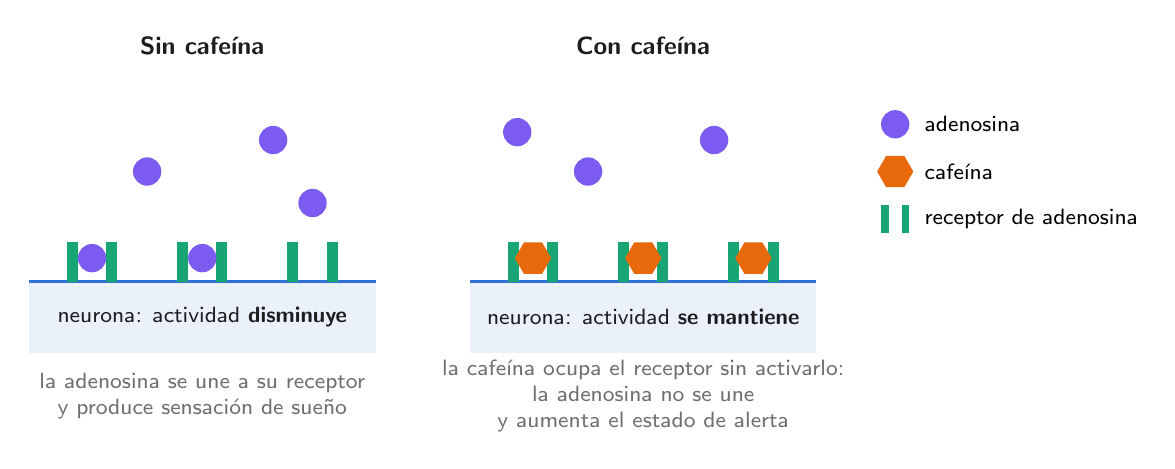
\begin{tikzpicture}[font=\footnotesize]
% panel 1
\node[font=\small\bfseries,text=tinta] at (2.2,3.0) {Sin cafeína};
\fill[azul!10] (0,-0.9) rectangle (4.4,0); \draw[azul,line width=1pt] (0,0) -- (4.4,0);
\foreach \x in {0.8,2.2,3.6}{\receptor{\x,0}}
\node[ade] at (0.8,0.3) {}; \node[ade] at (2.2,0.3) {};
\node[ade] at (1.5,1.4) {}; \node[ade] at (3.1,1.8) {}; \node[ade] at (3.6,1.0) {};
\node[align=center,text=tinta] at (2.2,-0.45) {neurona: actividad \textbf{disminuye}};
\node[align=center,text=gris] at (2.2,-1.45) {la adenosina se une a su receptor\\y produce sensación de sueño};
% panel 2
\begin{scope}[xshift=5.6cm]
\node[font=\small\bfseries,text=tinta] at (2.2,3.0) {Con cafeína};
\fill[azul!10] (0,-0.9) rectangle (4.4,0); \draw[azul,line width=1pt] (0,0) -- (4.4,0);
\foreach \x in {0.8,2.2,3.6}{\receptor{\x,0}}
\node[caf] at (0.8,0.3) {}; \node[caf] at (2.2,0.3) {}; \node[caf] at (3.6,0.3) {};
\node[ade] at (1.5,1.4) {}; \node[ade] at (3.1,1.8) {}; \node[ade] at (0.6,1.9) {};
\node[align=center,text=tinta] at (2.2,-0.45) {neurona: actividad \textbf{se mantiene}};
\node[align=center,text=gris] at (2.2,-1.45) {la cafeína ocupa el receptor sin activarlo:\\la adenosina no se une\\y aumenta el estado de alerta};
\end{scope}
% leyenda
\node[ade] at (11.0,2.0) {}; \node[anchor=west] at (11.25,2.0) {adenosina};
\node[caf] at (11.0,1.4) {}; \node[anchor=west] at (11.25,1.4) {cafeína};
\fill[menta] (10.82,0.62) rectangle ++(0.1,0.36); \fill[menta] (11.08,0.62) rectangle ++(0.1,0.36); \node[anchor=west] at (11.25,0.8) {receptor de adenosina};
\end{tikzpicture}
\end{document}
